\documentclass{beamer}
\usepackage[utf8]{inputenc}
\usepackage[T1]{fontenc}
\usepackage{graphicx}
\usepackage{amsmath}
\usepackage{amssymb}
\usepackage{xcolor}
\usepackage{tikz}
\usepackage{amsfonts}
\usepackage{algorithm, algorithmic}
\usepackage{multicol}
\usepackage{multirow}
\usetikzlibrary{shapes.geometric}
\usetheme{Copenhagen}
% \usetheme{metropolis}

\pdfmapfile{+packages/emerald/fonts/map/dvips/emerald.map}

\beamertemplatenavigationsymbolsempty

\setbeamertemplate{footline}{% 
  \hfill% 
  \usebeamercolor[fg]{page number in head/foot}% 
  \usebeamerfont{page number in head/foot}% 
  \insertframenumber%
  \kern1em\vskip2pt% 
}
\setbeamertemplate{headline}{}

\definecolor{bgcol}{RGB}{49,73,97}
\definecolor{bgcol2}{RGB}{0,24,55}


\setbeamercolor{block body}{bg=white}
\setbeamercolor{block title}{bg=bgcol2!90}
\setbeamercolor{frametitle}{bg=bgcol}
\setbeamercolor{frametitle}{fg=white}
\setbeamercolor{title}{bg=bgcol}
\setbeamercolor{title}{fg=white}
\setbeamercolor{section in toc}{bg=white}
\setbeamercolor{section in toc}{fg=black}
\setbeamercolor{subsection in toc}{bg=white}
\setbeamercolor{subsection in toc}{fg=black}
\setbeamercolor{subsubsection in toc}{bg=white}
\setbeamercolor{subsubsection in toc}{fg=black}
\setbeamertemplate{itemize item}{\color{black}$\blacksquare$}
\setbeamertemplate{itemize subitem}{\color{yellow}$\blacktriangleright$}

\defbeamertemplate{section in toc}{quadrado}
{\leavevmode\leftskip=1.75ex%
  \llap{%
    \usebeamerfont*{section number projected}%
    \usebeamercolor[black]{section number projected}%
    \vrule width2.7ex height2.12ex depth.58ex%
    \hskip-2.7ex%
    \hbox to2.7ex{\hfil\color{fg}\inserttocsectionnumber\hfil}}%
  \kern.3ex\inserttocsection\par}

\setbeamertemplate{section in toc}[quadrado]
\setcounter{tocdepth}{1}

\usebackgroundtemplate%
{%
    
\includegraphics[width=\paperwidth,height=\paperheight]{figures/bg4.JPG}%
}


\makeatletter
\setbeamertemplate{title}{
    \ifbeamercolorempty[bg]{title}{}{\nointerlineskip}%
    \@tempdima=\textwidth%
    \advance\@tempdima by\beamer@leftmargin%
    \advance\@tempdima by\beamer@rightmargin%
    \centering
    \begin{beamercolorbox}[sep=.5cm,wd=\the\@tempdima]{title}
        \centering
        \usebeamerfont{title}%
        \vbox{}\vskip-1ex%
        \if@tempswa\else\csname beamer@ftecenter\endcsname\fi%
        \strut\inserttitle\strut\par%
        {%
            \ifx\insertsubtitle\@empty%
            \else%
            {\usebeamerfont{subtitle}\usebeamercolor[fg]{subtitle}\insertsubtitle\strut\par}%
            \fi
        }%
        \vskip-1ex%
        \if@tempswa\else\vskip-.3cm\fi
    \end{beamercolorbox}%
}

\setbeamertemplate{frametitle}{
    \ifbeamercolorempty[bg]{frametitle}{}{\nointerlineskip}%
    \@tempdima=\textwidth%
    \advance\@tempdima by\beamer@leftmargin%
    \advance\@tempdima by\beamer@rightmargin%
    \vspace*{1.2cm} 
    % \hspace*{0cm}
    \begin{beamercolorbox}[sep=0.3cm,wd=\the\@tempdima]{frametitle}
        \usebeamerfont{frametitle}%
        \vbox{}\vskip-1ex%
        \if@tempswa\else\csname beamer@ftecenter\endcsname\fi%
        \strut\insertframetitle\strut\par%
        {%
            \ifx\insertframesubtitle\@empty%
            \else%
            {\usebeamerfont{framesubtitle}\usebeamercolor[fg]{framesubtitle}\insertframesubtitle\strut\par}%
            \fi
        }%
        \vskip-1ex%
        \if@tempswa\else\vskip-.3cm\fi
    \end{beamercolorbox}%
}
\makeatother

\title{Randomized Algorithms}
\subtitle{Monte Carlo Algorithm}
\author {
    Farriha Afnan - 2005061\\
    Abrar Rahman Abir - 2005072\\
    Ananya Shahrin Promi - 2005079\\
}
\institute{Department of CSE,\\ Bangladesh University of Engineering and Technology} 
\date{February 20, 2024}

\AtBeginSection
{
    \begin{frame}
	\frametitle{Contents}
        \begin{columns}[t]
            \begin{column}{.2\textwidth}
            \end{column}
            \begin{column}{.8\textwidth}
                \tableofcontents[currentsection]
            \end{column}
        \end{columns}
    \end{frame}
}

\begin{document}
    \nocite{MITOCWCourse}
    \nocite{MC}
    \nocite{MCS}

    \begin{frame}
        \titlepage
    \end{frame}
    
    \begin{frame}{Overview}
        \begin{columns}[t]
            \begin{column}{.2\textwidth}
            \end{column}
            \begin{column}{.8\textwidth}
                \tableofcontents
            \end{column}
        \end{columns}
    \end{frame}

    \section{Introduction}
    \begin{frame}{Introduction}
        \begin{block}{What is Randomized Algorithm?}
            A randomized algorithm is defined as an algorithm that receives a stream of random bits in addition to its input. It utilizes this stream for making random choices during its execution.
        \end{block}
    \end{frame}

    \subsection{Classification}
    \begin{frame}{Las Vegas and Monte Carlo}
        \begin{block}{Las Vegas Algorithm}
            It constitutes those randomized algorithms that always give a correct answer, or do not give an answer.
        \end{block}
        \begin{block}{Monte Carlo Algorithm}
            It always answers, but may occasionally produce an incorrect answer. The probability of producing an incorrect answer can be made arbitrarily small by running the algorithm repeatedly with independent random choices.
        \end{block}
    \end{frame}

    \section{Unveiling Monte Carlo}
    \begin{frame}{Beyond the Casino's Games of Chance}
    \vspace{2em}
    The name \textit{Monte Carlo} comes from the Monte Carlo Casino in Monaco, known for its games of chance and randomness.
        \begin{figure}
            \centering
            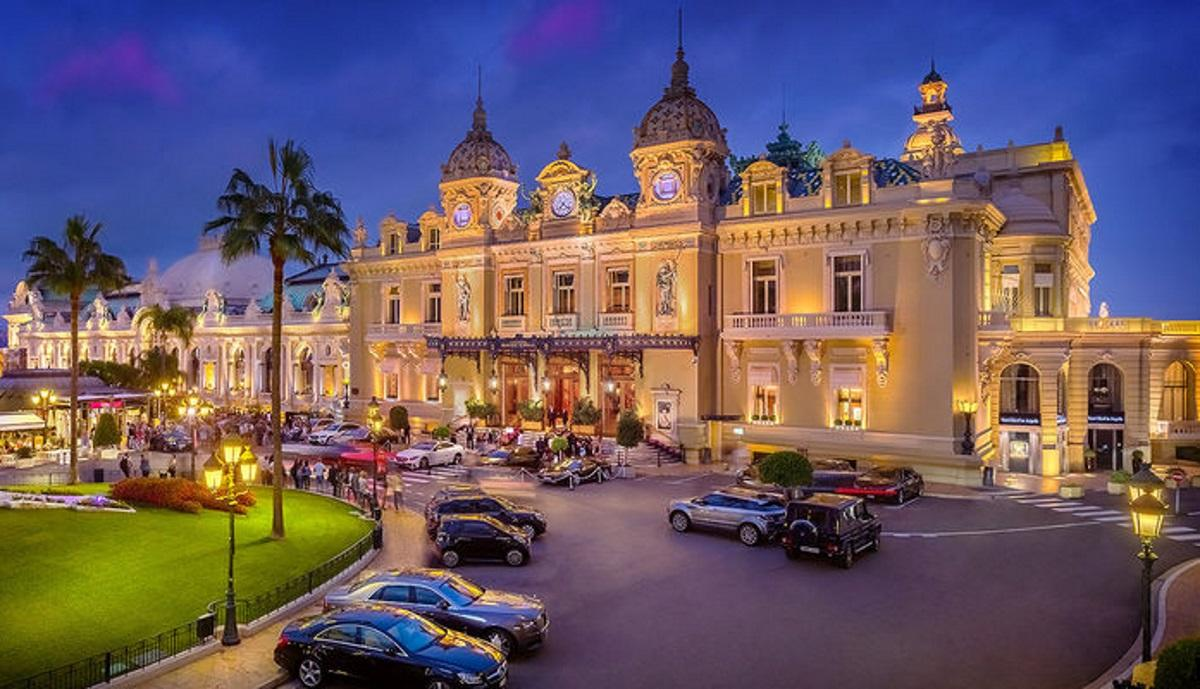
\includegraphics[width=0.5\textwidth]{figures/casino.jpg}
            \caption{Casino de Monte-Carlo}
            \label{fig:casino}
        \end{figure}
    \end{frame}

    \subsection{History}
    \begin{frame}{A Little History}
        \begin{itemize}
            \item Stanislaw Ulam, recovering from an illness, was playing a lot of solitaire
            \item Tried to figure out the probability of winning but failed
            \item Thought about playing lots of hands and counting the number of wins but it would take years
            \item Asked Von Neumann if he could build a program to simulate many hands on ENIAC
        \end{itemize}
    \end{frame}

    \section{Monte Carlo Simulation}
    \begin{frame}{Monte Carlo Simulation}
        \begin{block}{About Monte Carlo}
            \begin{itemize}
                \item A method of estimating the value of an unknown quantity using the principles of inferential statistics
                \item Inferential Statistics
                \begin{itemize}
                    \item[] \textbf{Population:} a set of examples
    ◦               \item[] \textbf{Sample:} a proper subset of a population 
                \end{itemize}
            \end{itemize}
            \vspace{1em}
        \end{block}
        \vspace{1em}
        % \begin{block}{Key fact}
        %     A random sample tends to exhibit the same properties as the population from which it is drawn
        % \end{block}
    \end{frame}

    \subsection{Example}
    \begin{frame}{An Example}
        \begin{center}
            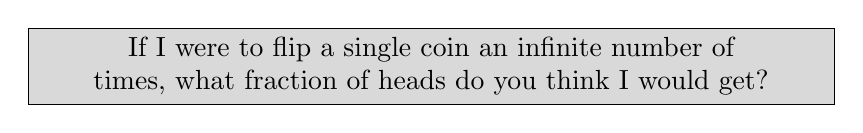
\begin{tikzpicture}
                \node[draw, rectangle, black, fill=gray!30, text width = 10cm, text centered]{If I were to flip a single coin an infinite number of times, what fraction of heads do you think I would get?};
            \end{tikzpicture}
        \end{center}
    \end{frame}
    
    \begin{frame}{Consider One Flip}
        \begin{figure}
            \centering
            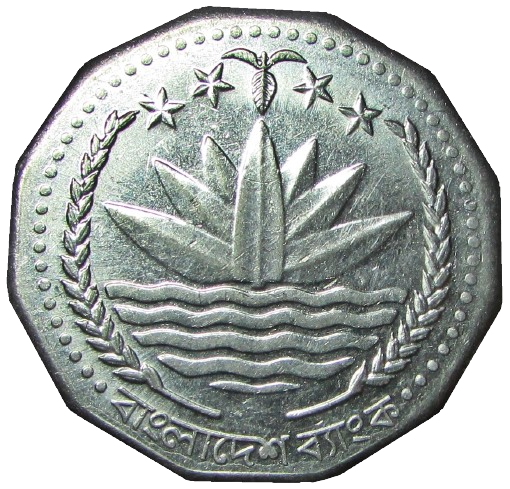
\includegraphics[scale=0.2]{figures/coin.png}
        \end{figure}
        \begin{center}
            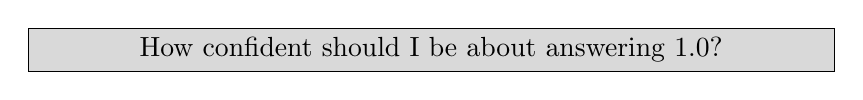
\begin{tikzpicture}
                \node[draw, rectangle, black, fill=gray!30, text width = 10cm, text centered]{How confident should I be about answering 1.0?};
            \end{tikzpicture}
        \end{center}
    \end{frame}

    \begin{frame}{Consider Two Flips}
        \begin{table}[h]
            \centering
            \begin{tabular}{cc}
                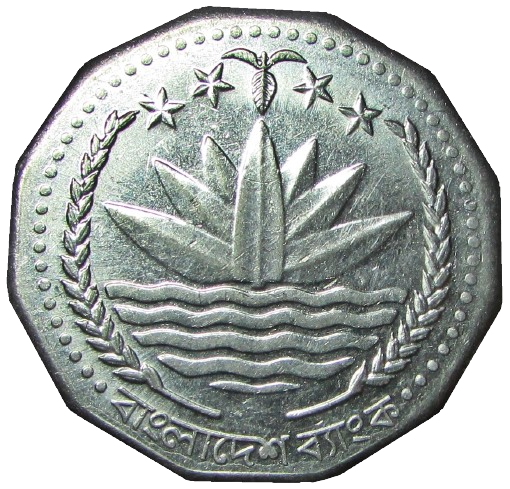
\includegraphics[scale=0.15]{figures/coin.png} & 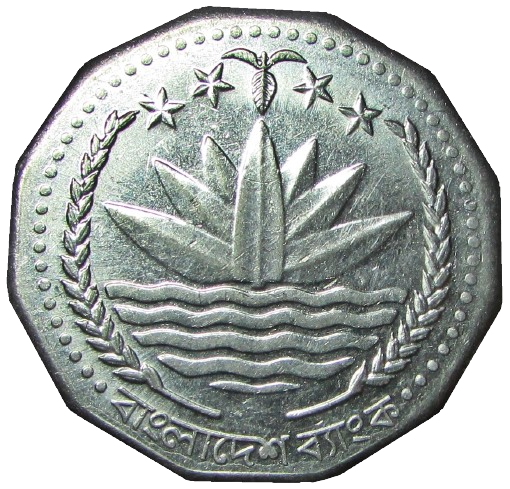
\includegraphics[scale=0.15]{figures/coin.png}\\
            \end{tabular}
        \end{table}
        \begin{center}
            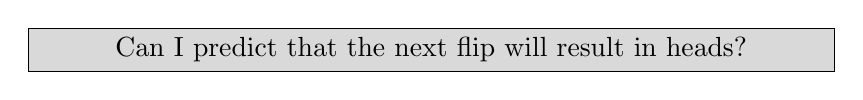
\begin{tikzpicture}
                \node[draw, rectangle, black, fill=gray!30, text width = 10cm, text centered]{Can I predict that the next flip will result in heads?};
            \end{tikzpicture}
        \end{center}
    \end{frame}

    \begin{frame}{Consider Hundred Flips}
        \begin{table}[h]
            \centering
            \begin{tabular}{c@{\hspace{.5em}}c@{\hspace{.5em}}c@{\hspace{.5em}}c@{\hspace{.5em}}c@{\hspace{.5em}}c@{\hspace{.5em}}c@{\hspace{.5em}}c@{\hspace{.5em}}c@{\hspace{.5em}}c}
                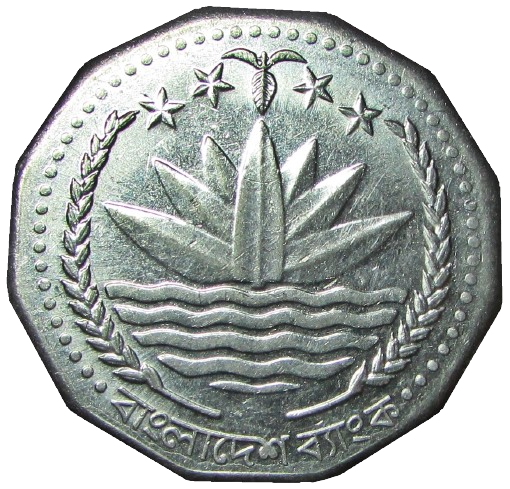
\includegraphics[scale=0.02]{figures/coin.png} & 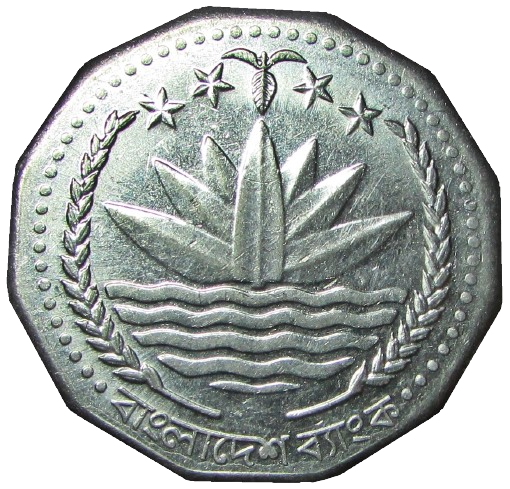
\includegraphics[scale=0.02]{figures/coin.png} & 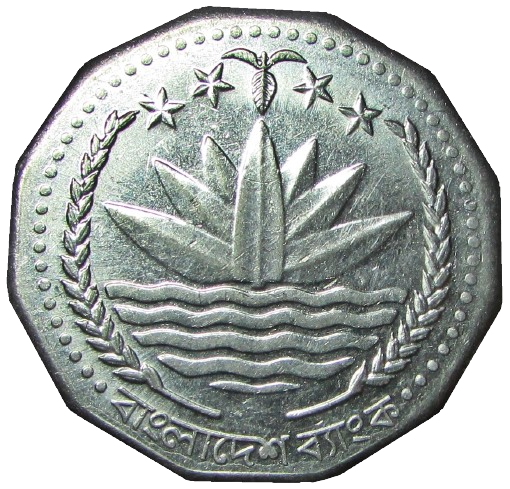
\includegraphics[scale=0.02]{figures/coin.png} & 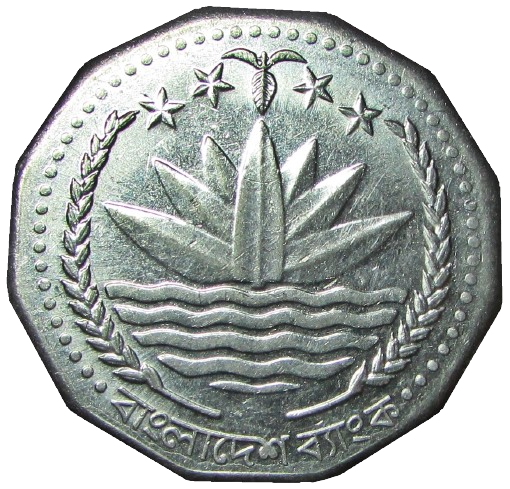
\includegraphics[scale=0.02]{figures/coin.png} & 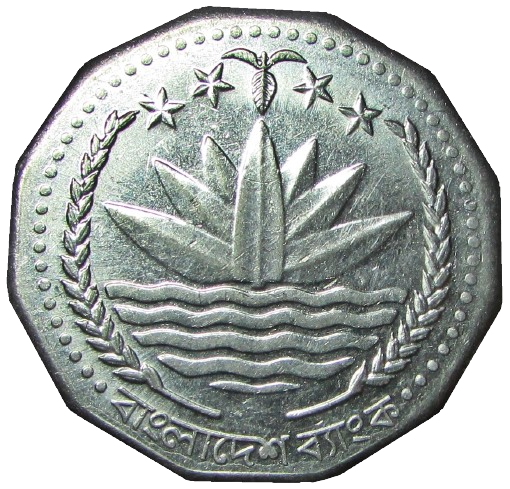
\includegraphics[scale=0.02]{figures/coin.png} & 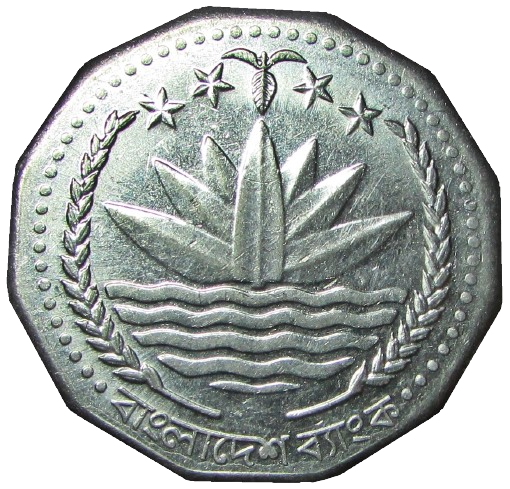
\includegraphics[scale=0.02]{figures/coin.png} &
                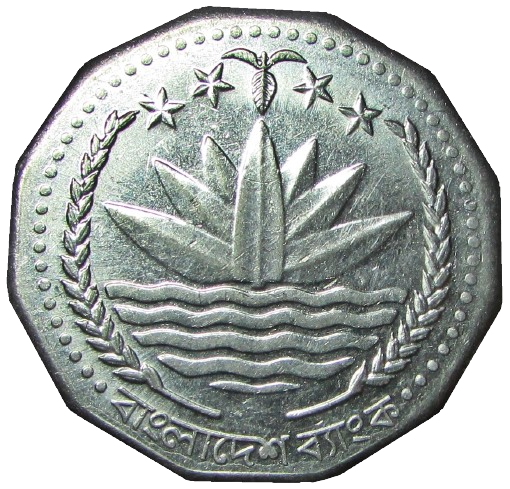
\includegraphics[scale=0.02]{figures/coin.png} & 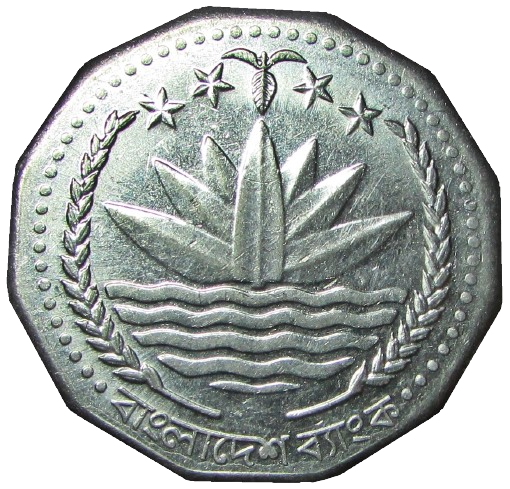
\includegraphics[scale=0.02]{figures/coin.png} &
                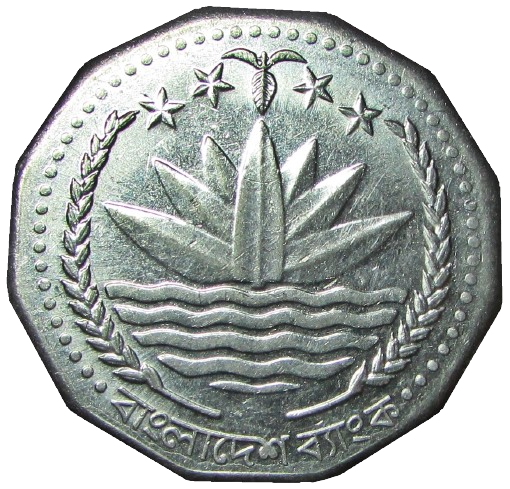
\includegraphics[scale=0.02]{figures/coin.png} & 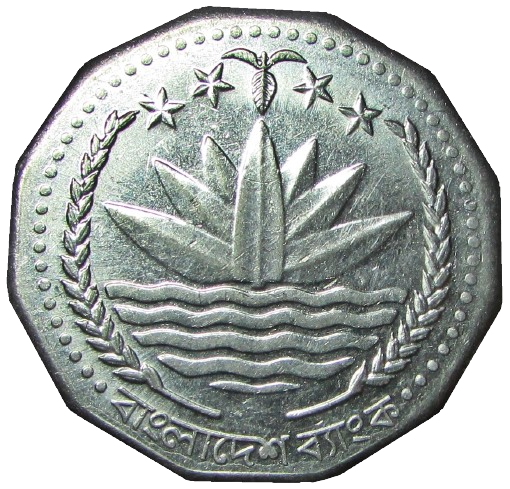
\includegraphics[scale=0.02]{figures/coin.png}\\
                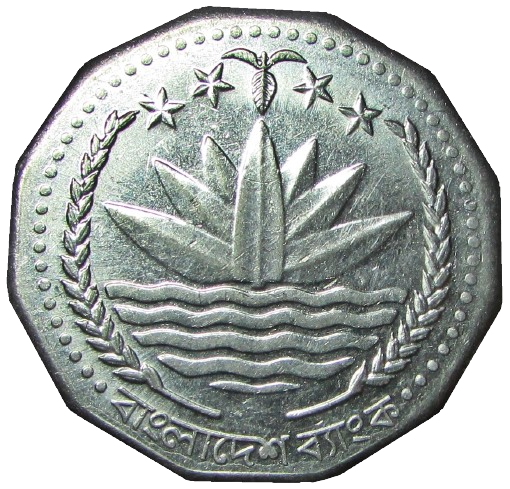
\includegraphics[scale=0.02]{figures/coin.png} & 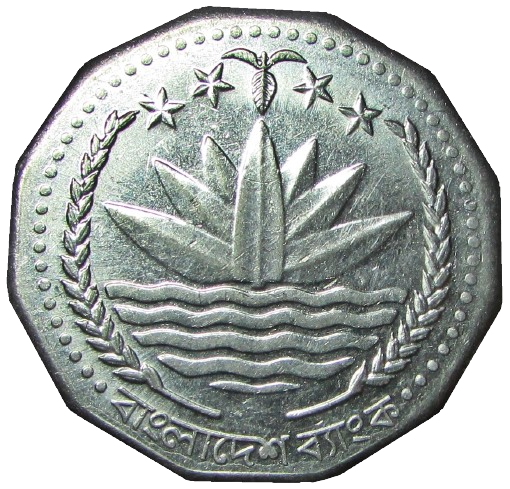
\includegraphics[scale=0.02]{figures/coin.png} & 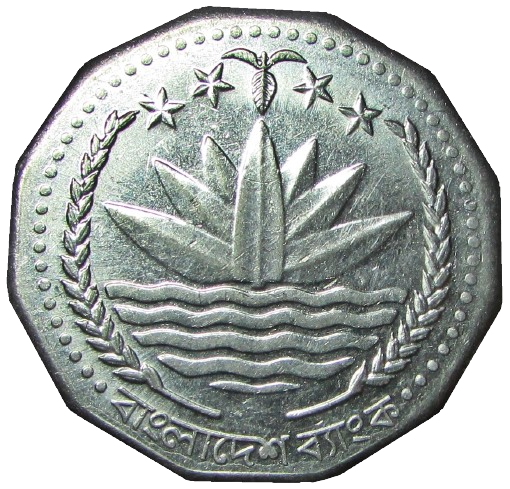
\includegraphics[scale=0.02]{figures/coin.png} & 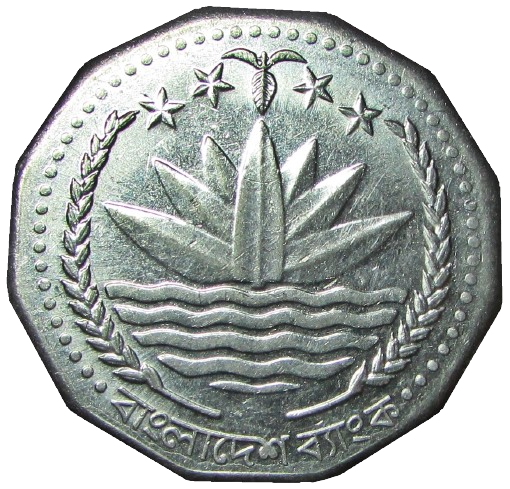
\includegraphics[scale=0.02]{figures/coin.png} & 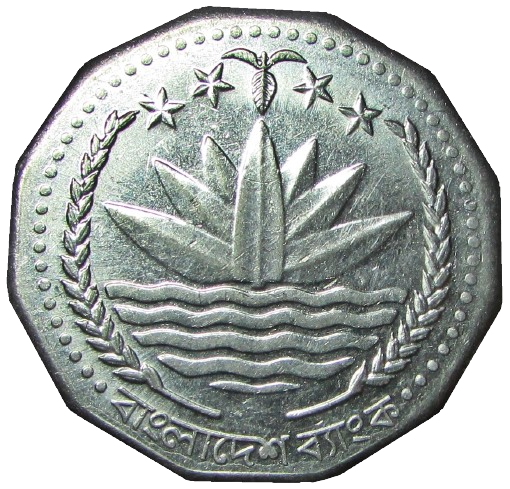
\includegraphics[scale=0.02]{figures/coin.png} & 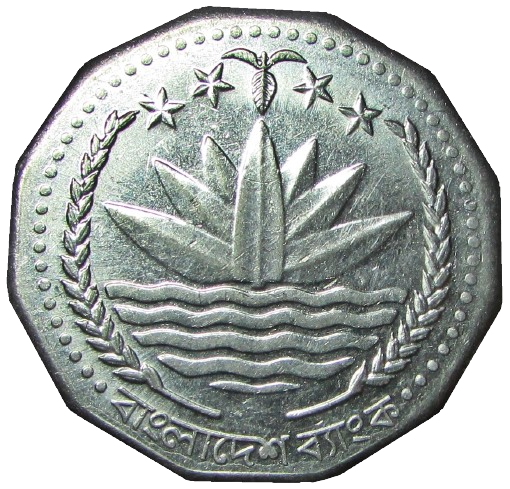
\includegraphics[scale=0.02]{figures/coin.png} &
                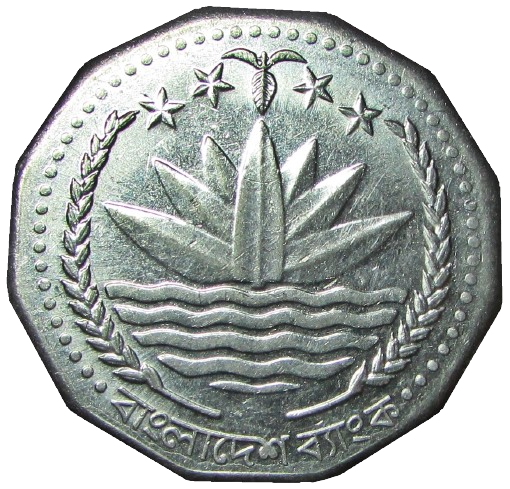
\includegraphics[scale=0.02]{figures/coin.png} & 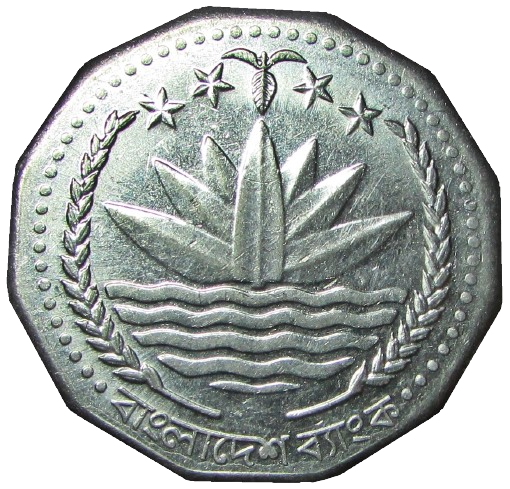
\includegraphics[scale=0.02]{figures/coin.png} &
                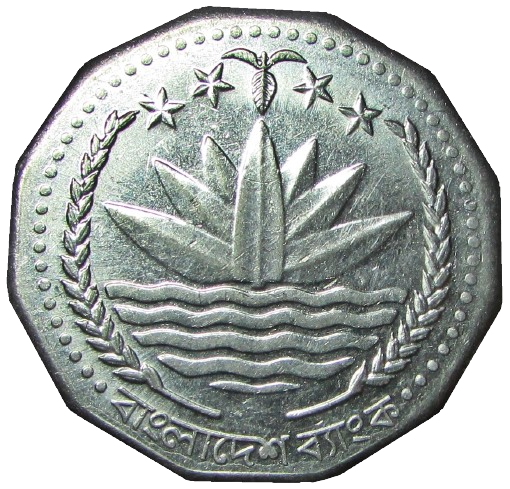
\includegraphics[scale=0.02]{figures/coin.png} & 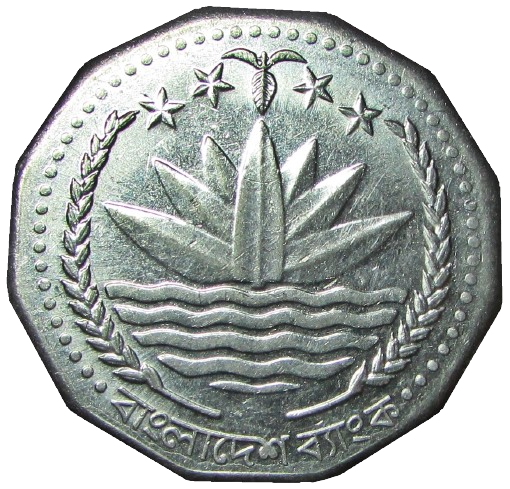
\includegraphics[scale=0.02]{figures/coin.png}\\
                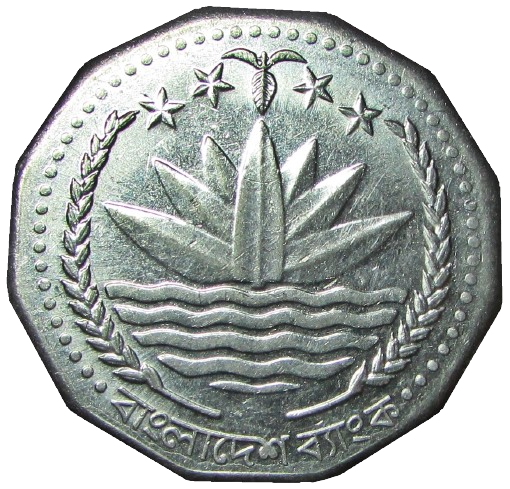
\includegraphics[scale=0.02]{figures/coin.png} & 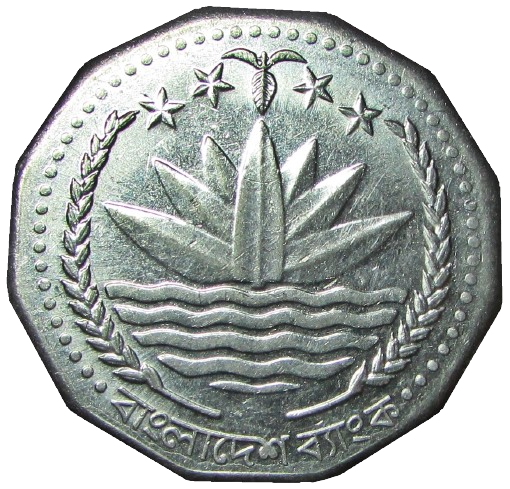
\includegraphics[scale=0.02]{figures/coin.png} & 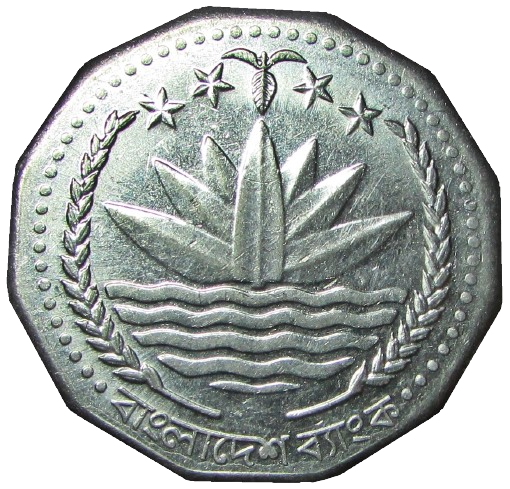
\includegraphics[scale=0.02]{figures/coin.png} & 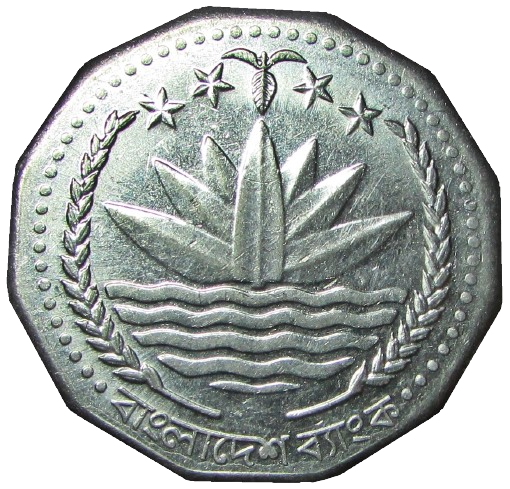
\includegraphics[scale=0.02]{figures/coin.png} & 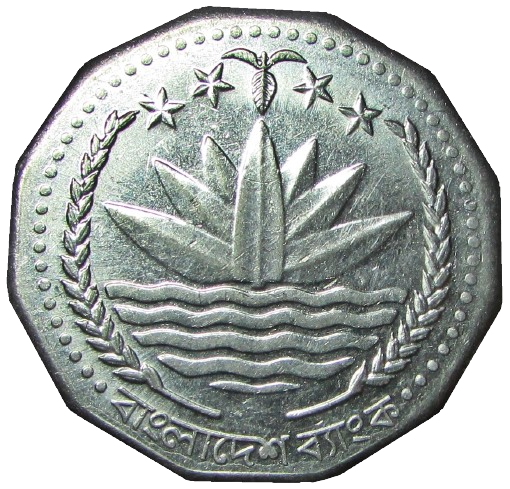
\includegraphics[scale=0.02]{figures/coin.png} & 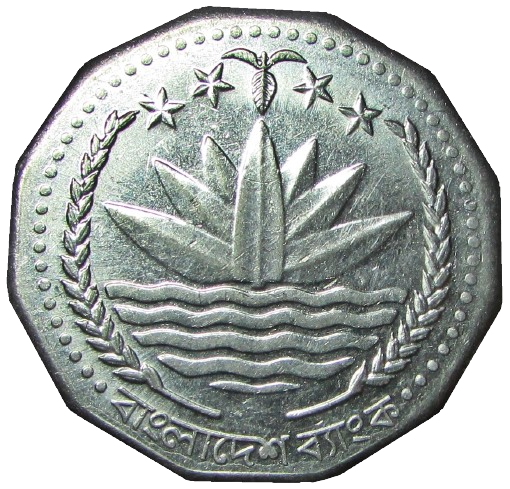
\includegraphics[scale=0.02]{figures/coin.png} &
                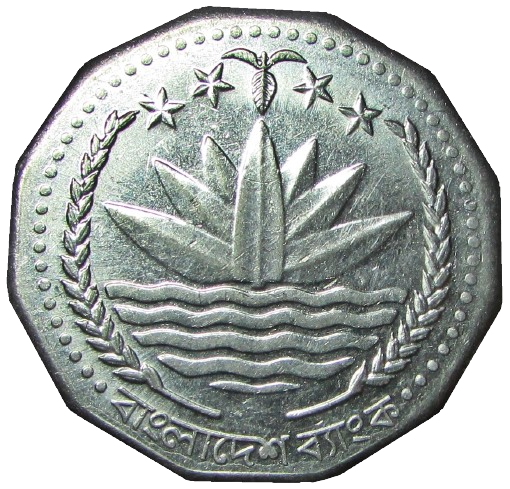
\includegraphics[scale=0.02]{figures/coin.png} & 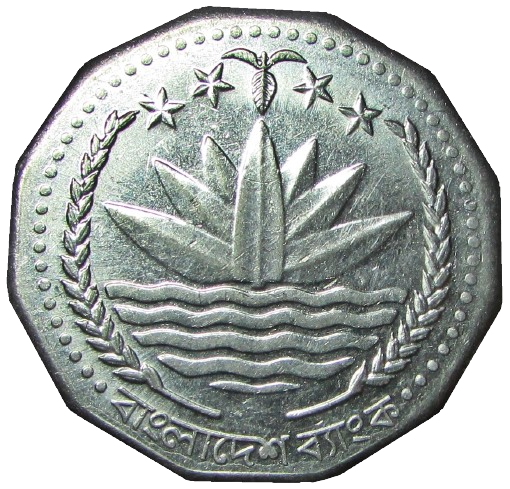
\includegraphics[scale=0.02]{figures/coin.png} &
                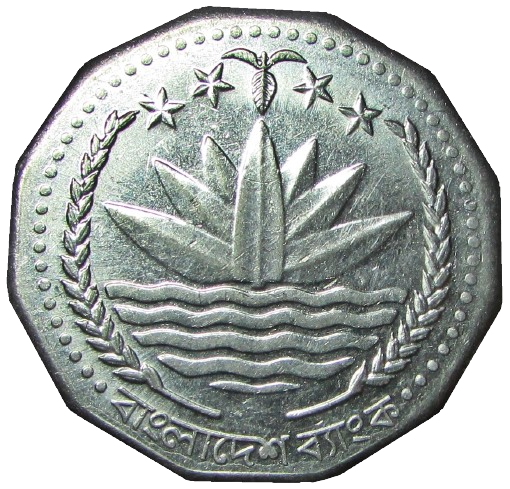
\includegraphics[scale=0.02]{figures/coin.png} & 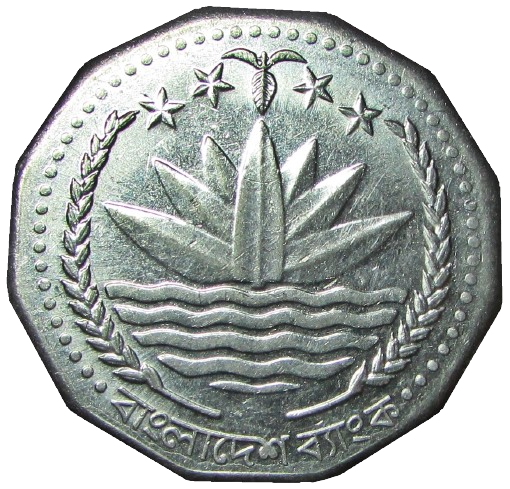
\includegraphics[scale=0.02]{figures/coin.png}\\
                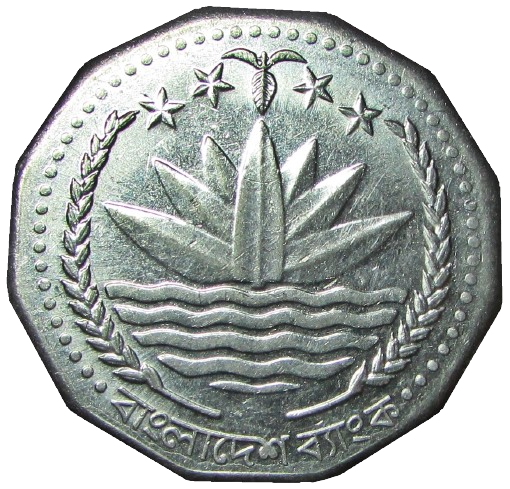
\includegraphics[scale=0.02]{figures/coin.png} & 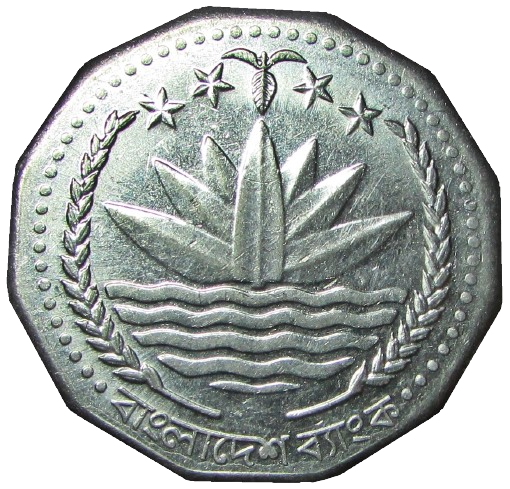
\includegraphics[scale=0.02]{figures/coin.png} & 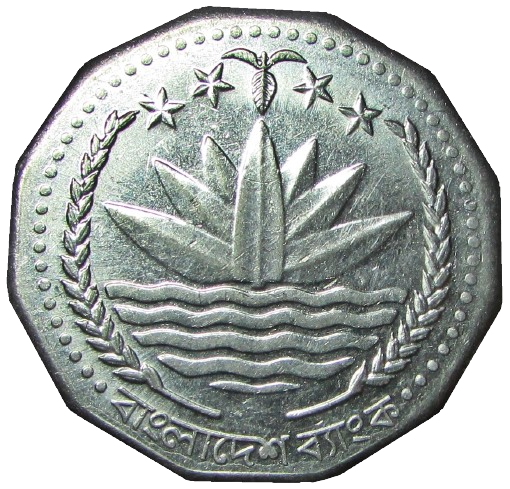
\includegraphics[scale=0.02]{figures/coin.png} & 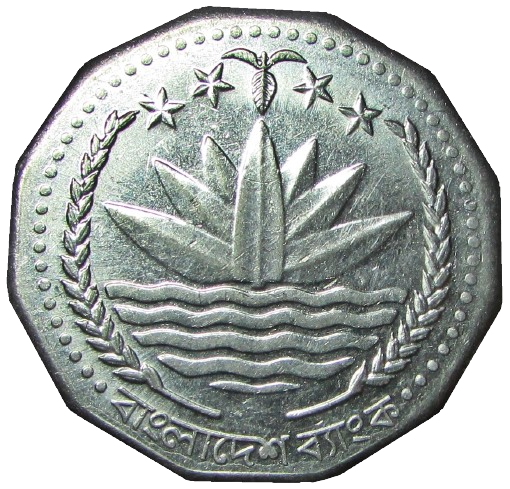
\includegraphics[scale=0.02]{figures/coin.png} & 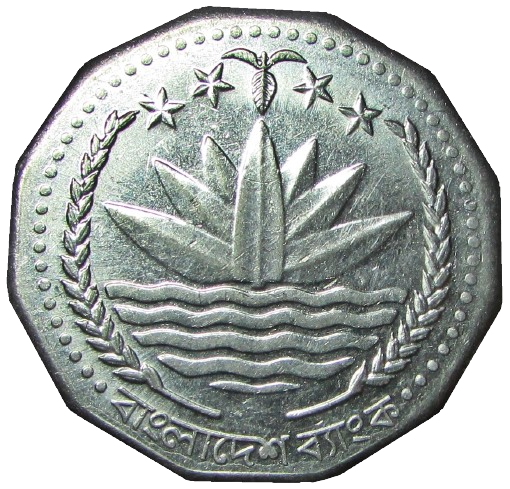
\includegraphics[scale=0.02]{figures/coin.png} & 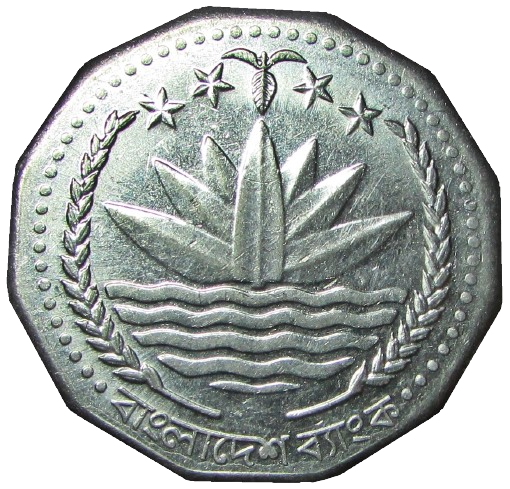
\includegraphics[scale=0.02]{figures/coin.png} &
                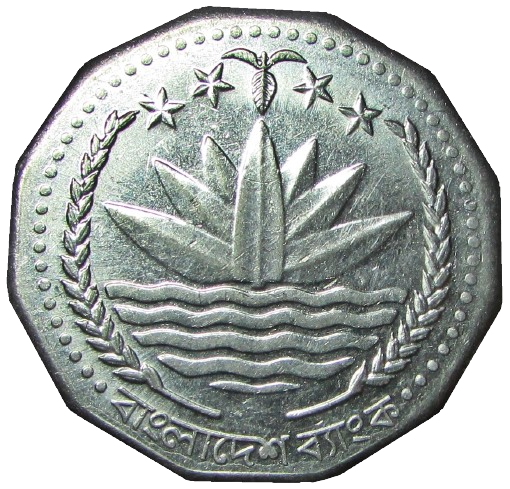
\includegraphics[scale=0.02]{figures/coin.png} & 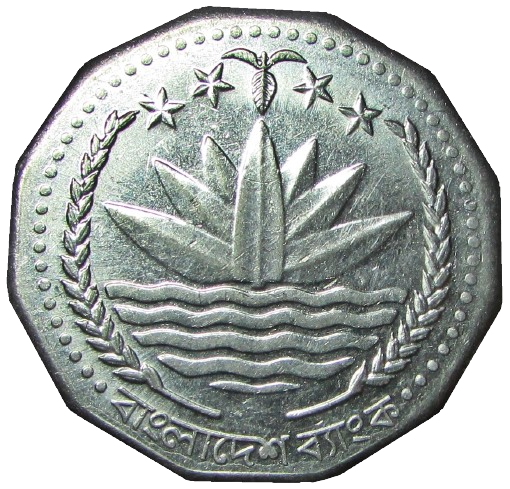
\includegraphics[scale=0.02]{figures/coin.png} &
                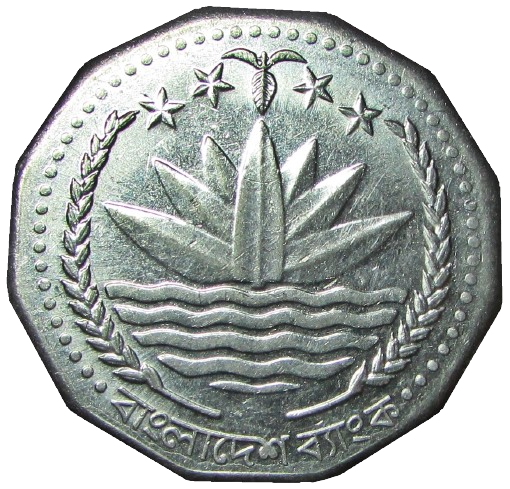
\includegraphics[scale=0.02]{figures/coin.png} & 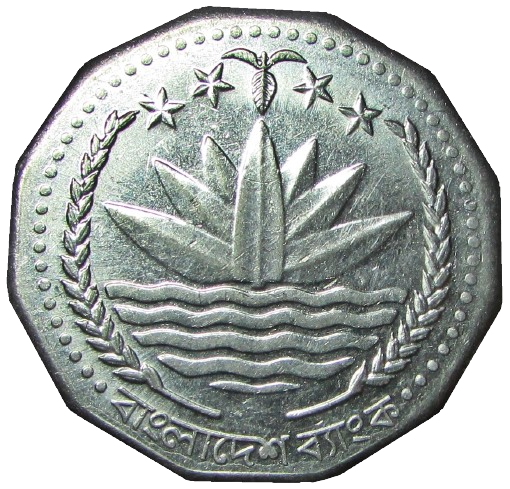
\includegraphics[scale=0.02]{figures/coin.png}\\
                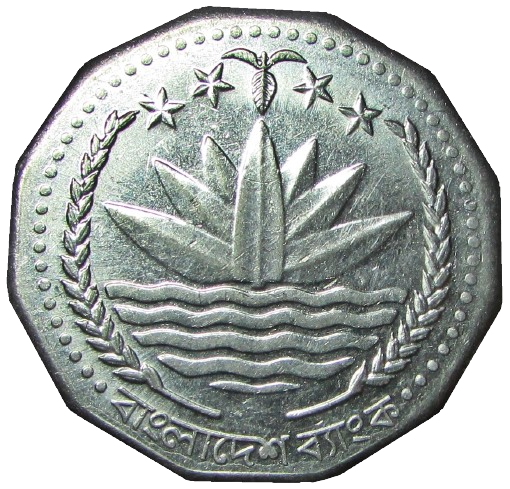
\includegraphics[scale=0.02]{figures/coin.png} & 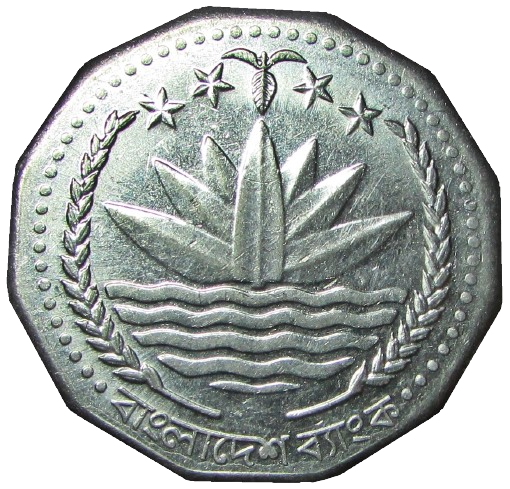
\includegraphics[scale=0.02]{figures/coin.png} & 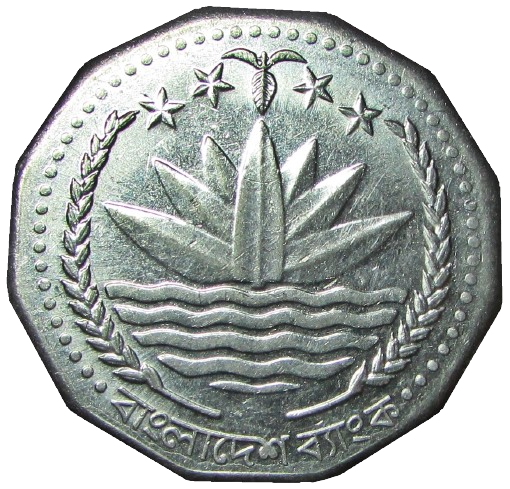
\includegraphics[scale=0.02]{figures/coin.png} & 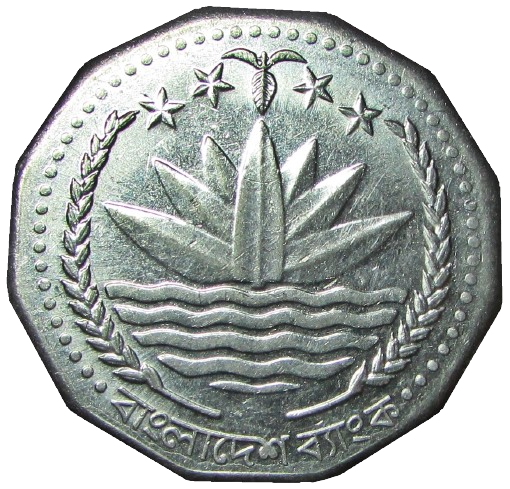
\includegraphics[scale=0.02]{figures/coin.png} & 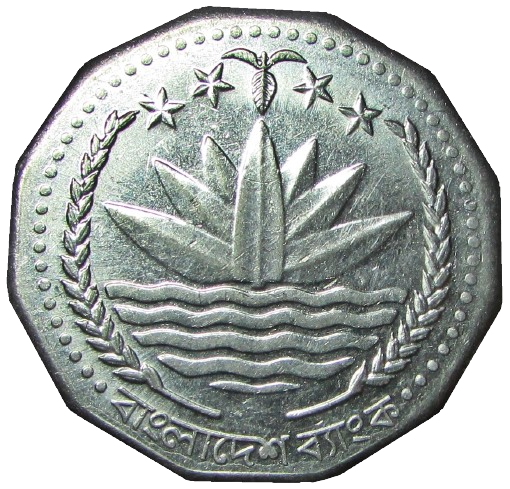
\includegraphics[scale=0.02]{figures/coin.png} & \includegraphics[scale=0.02]{figures/coin.png} &
                \includegraphics[scale=0.02]{figures/coin.png} & \includegraphics[scale=0.02]{figures/coin.png} &
                \includegraphics[scale=0.02]{figures/coin.png} & \includegraphics[scale=0.02]{figures/coin.png}\\
                \includegraphics[scale=0.02]{figures/coin.png} & \includegraphics[scale=0.02]{figures/coin.png} & \includegraphics[scale=0.02]{figures/coin.png} & \includegraphics[scale=0.02]{figures/coin.png} & \includegraphics[scale=0.02]{figures/coin.png} & \includegraphics[scale=0.02]{figures/coin.png} &
                \includegraphics[scale=0.02]{figures/coin.png} & \includegraphics[scale=0.02]{figures/coin.png} &
                \includegraphics[scale=0.02]{figures/coin.png} & \includegraphics[scale=0.02]{figures/coin.png}\\
                \includegraphics[scale=0.02]{figures/coin.png} & \includegraphics[scale=0.02]{figures/coin.png} & \includegraphics[scale=0.02]{figures/coin.png} & \includegraphics[scale=0.02]{figures/coin.png} & \includegraphics[scale=0.02]{figures/coin.png} & \includegraphics[scale=0.02]{figures/coin.png} &
                \includegraphics[scale=0.02]{figures/coin.png} & \includegraphics[scale=0.02]{figures/coin.png} &
                \includegraphics[scale=0.02]{figures/coin.png} & \includegraphics[scale=0.02]{figures/coin.png}\\
                \includegraphics[scale=0.02]{figures/coin.png} & \includegraphics[scale=0.02]{figures/coin.png} & \includegraphics[scale=0.02]{figures/coin.png} & \includegraphics[scale=0.02]{figures/coin.png} & \includegraphics[scale=0.02]{figures/coin.png} & \includegraphics[scale=0.02]{figures/coin.png} &
                \includegraphics[scale=0.02]{figures/coin.png} & \includegraphics[scale=0.02]{figures/coin.png} &
                \includegraphics[scale=0.02]{figures/coin.png} & \includegraphics[scale=0.02]{figures/coin.png}\\
                \includegraphics[scale=0.02]{figures/coin.png} & \includegraphics[scale=0.02]{figures/coin.png} & \includegraphics[scale=0.02]{figures/coin.png} & \includegraphics[scale=0.02]{figures/coin.png} & \includegraphics[scale=0.02]{figures/coin.png} & \includegraphics[scale=0.02]{figures/coin.png} &
                \includegraphics[scale=0.02]{figures/coin.png} & \includegraphics[scale=0.02]{figures/coin.png} &
                \includegraphics[scale=0.02]{figures/coin.png} & \includegraphics[scale=0.02]{figures/coin.png}\\
                \includegraphics[scale=0.02]{figures/coin.png} & \includegraphics[scale=0.02]{figures/coin.png} & \includegraphics[scale=0.02]{figures/coin.png} & \includegraphics[scale=0.02]{figures/coin.png} & \includegraphics[scale=0.02]{figures/coin.png} & \includegraphics[scale=0.02]{figures/coin.png} &
                \includegraphics[scale=0.02]{figures/coin.png} & \includegraphics[scale=0.02]{figures/coin.png} &
                \includegraphics[scale=0.02]{figures/coin.png} & \includegraphics[scale=0.02]{figures/coin.png}\\
            \end{tabular}
        \end{table}
        \begin{center}
            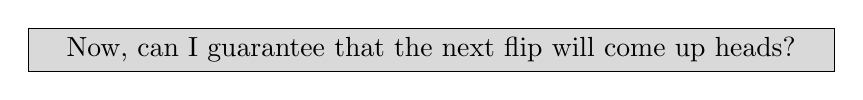
\begin{tikzpicture}
                \node[draw, rectangle, black, fill=gray!30, text width = 10cm, text centered]{Now, can I guarantee that the next flip will come up heads?};
            \end{tikzpicture}
        \end{center}
    \end{frame}

    \begin{frame}{Consider Hundred Flips}
        \begin{table}[h]
            \centering
            \begin{tabular}{c@{\hspace{.5em}}c@{\hspace{.5em}}c@{\hspace{.5em}}c@{\hspace{.5em}}c@{\hspace{.5em}}c@{\hspace{.5em}}c@{\hspace{.5em}}c@{\hspace{.5em}}c@{\hspace{.5em}}c}
                \includegraphics[scale=0.02]{figures/coin.png} & \includegraphics[scale=0.02]{figures/coin.png} & \includegraphics[scale=0.02]{figures/coin.png} & \includegraphics[scale=0.02]{figures/coin.png} & \includegraphics[scale=0.02]{figures/coin.png} & \includegraphics[scale=0.02]{figures/coin.png} &
                \includegraphics[scale=0.02]{figures/coin.png} & \includegraphics[scale=0.02]{figures/coin.png} &
                \includegraphics[scale=0.02]{figures/coin.png} & \includegraphics[scale=0.02]{figures/coin.png}\\
                \includegraphics[scale=0.02]{figures/coin.png} & \includegraphics[scale=0.02]{figures/coin.png} & \includegraphics[scale=0.02]{figures/coin.png} & \includegraphics[scale=0.02]{figures/coin.png} & \includegraphics[scale=0.02]{figures/coin.png} & \includegraphics[scale=0.02]{figures/coin.png} &
                \includegraphics[scale=0.02]{figures/coin.png} & \includegraphics[scale=0.02]{figures/coin.png} &
                \includegraphics[scale=0.02]{figures/coin.png} & \includegraphics[scale=0.02]{figures/coin.png}\\
                \includegraphics[scale=0.02]{figures/coin.png} & \includegraphics[scale=0.02]{figures/coin.png} & \includegraphics[scale=0.02]{figures/coin.png} & \includegraphics[scale=0.02]{figures/coin.png} & \includegraphics[scale=0.02]{figures/coin.png} & \includegraphics[scale=0.02]{figures/coin.png} &
                \includegraphics[scale=0.02]{figures/coin.png} & \includegraphics[scale=0.02]{figures/coin.png} &
                \includegraphics[scale=0.02]{figures/coin.png} & \includegraphics[scale=0.02]{figures/coin.png}\\
                \includegraphics[scale=0.02]{figures/coin.png} & \includegraphics[scale=0.02]{figures/coin.png} & \includegraphics[scale=0.02]{figures/coin.png} & \includegraphics[scale=0.02]{figures/coin.png} & \includegraphics[scale=0.02]{figures/coin.png} & \includegraphics[scale=0.02]{figures/coin.png} &
                \includegraphics[scale=0.02]{figures/coin.png} & \includegraphics[scale=0.02]{figures/coin.png} &
                \includegraphics[scale=0.02]{figures/coin.png} & \includegraphics[scale=0.02]{figures/coin.png}\\
                \includegraphics[scale=0.02]{figures/coin.png} & \includegraphics[scale=0.02]{figures/coin.png} & \includegraphics[scale=0.02]{figures/coin.png} & \includegraphics[scale=0.02]{figures/coin.png} & \includegraphics[scale=0.02]{figures/coin.png} & \includegraphics[scale=0.02]{figures/coin.png} &
                \includegraphics[scale=0.02]{figures/coin.png} & \includegraphics[scale=0.02]{figures/coin.png} &
                \includegraphics[scale=0.02]{figures/coin.png} & \includegraphics[scale=0.02]{figures/coin.png}\\
                \includegraphics[scale=0.02]{figures/coin.png} & \includegraphics[scale=0.02]{figures/coin.png} & \includegraphics[scale=0.02]{figures/coint.png} & \includegraphics[scale=0.02]{figures/coint.png} & \includegraphics[scale=0.02]{figures/coint.png} & \includegraphics[scale=0.02]{figures/coint.png} &
                \includegraphics[scale=0.02]{figures/coint.png} & \includegraphics[scale=0.02]{figures/coint.png} &
                \includegraphics[scale=0.02]{figures/coint.png} & \includegraphics[scale=0.02]{figures/coint.png}\\
                \includegraphics[scale=0.02]{figures/coint.png} & \includegraphics[scale=0.02]{figures/coint.png} & \includegraphics[scale=0.02]{figures/coint.png} & \includegraphics[scale=0.02]{figures/coint.png} & \includegraphics[scale=0.02]{figures/coint.png} & \includegraphics[scale=0.02]{figures/coint.png} &
                \includegraphics[scale=0.02]{figures/coint.png} & \includegraphics[scale=0.02]{figures/coint.png} &
                \includegraphics[scale=0.02]{figures/coint.png} & \includegraphics[scale=0.02]{figures/coint.png}\\
                \includegraphics[scale=0.02]{figures/coint.png} & \includegraphics[scale=0.02]{figures/coint.png} & \includegraphics[scale=0.02]{figures/coint.png} & \includegraphics[scale=0.02]{figures/coint.png} & \includegraphics[scale=0.02]{figures/coint.png} & \includegraphics[scale=0.02]{figures/coint.png} &
                \includegraphics[scale=0.02]{figures/coint.png} & \includegraphics[scale=0.02]{figures/coint.png} &
                \includegraphics[scale=0.02]{figures/coint.png} & \includegraphics[scale=0.02]{figures/coint.png}\\
                \includegraphics[scale=0.02]{figures/coint.png} & \includegraphics[scale=0.02]{figures/coint.png} & \includegraphics[scale=0.02]{figures/coint.png} & \includegraphics[scale=0.02]{figures/coint.png} & \includegraphics[scale=0.02]{figures/coint.png} & \includegraphics[scale=0.02]{figures/coint.png} &
                \includegraphics[scale=0.02]{figures/coint.png} & \includegraphics[scale=0.02]{figures/coint.png} &
                \includegraphics[scale=0.02]{figures/coint.png} & \includegraphics[scale=0.02]{figures/coint.png}\\
                \includegraphics[scale=0.02]{figures/coint.png} & \includegraphics[scale=0.02]{figures/coint.png} & \includegraphics[scale=0.02]{figures/coint.png} & \includegraphics[scale=0.02]{figures/coint.png} & \includegraphics[scale=0.02]{figures/coint.png} & \includegraphics[scale=0.02]{figures/coint.png} &
                \includegraphics[scale=0.02]{figures/coint.png} & \includegraphics[scale=0.02]{figures/coint.png} &
                \includegraphics[scale=0.02]{figures/coint.png} & \includegraphics[scale=0.02]{figures/coint.png}\\
            \end{tabular}
        \end{table}
        \begin{center}
            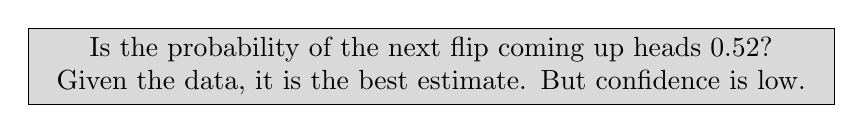
\begin{tikzpicture}
                \node[draw, rectangle, black, fill=gray!30, text width = 10cm, text centered]{Is the probability of the next flip coming up heads 0.52? Given the data, it is the best estimate. But confidence is low.};
            \end{tikzpicture}
        \end{center}
    \end{frame}

    \begin{frame}{Difference in Confidence}
    \begin{center}
            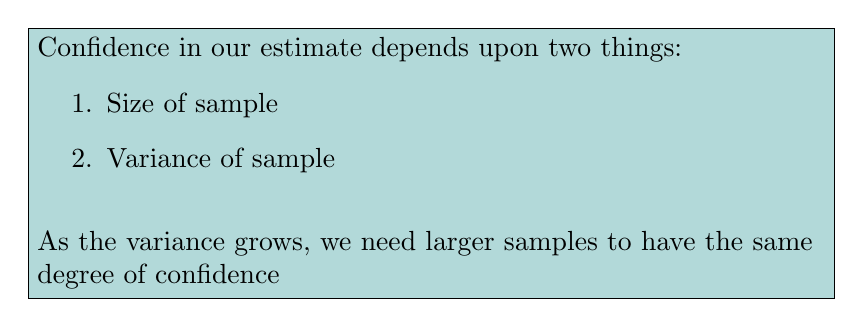
\begin{tikzpicture}
                \node[draw, rectangle, black, fill=teal!30, text width = 10cm]{Confidence in our estimate depends upon two things:
        \begin{enumerate}
            \item Size of sample
            \item Variance of sample
        \end{enumerate}
        \vspace{1em}
        As the variance grows, we need larger samples to have the same degree of confidence};
            \end{tikzpicture}
        \end{center}
    \end{frame}

    % \section{Law of Large Numbers}
    % \begin{frame}{Law of Large Numbers}
    %     \begin{center}
    %         \begin{tikzpicture}
    %             \node<1->[draw, rectangle, black, fill=pink!10, text width = 10cm](no1){In repeated independent tests with the same actual probability \textit{p} of a particular outcome in each test, the chance that the fraction of times that outcome occurs differs from \textit{p} converges to zero as the number of trials goes to infinity.};
    %             \node<2->[draw, rectangle, black, fill=violet!10, text width = 10.5cm, below of=no1, yshift=-2cm]{Does this imply that if deviations from expected behavior occur, these deviations are likely to be evened out by opposite deviations in the future?};
    %         \end{tikzpicture}
    %     \end{center}
    % \end{frame}

    % \subsection{Regression and Mean}
    % \begin{frame}{Regression to the Mean}
    %     \begin{block}<1->{Extreme Random Event}
    %         If you toss a fair coin 10 times and get 100\% heads, that is an extreme event
    %     \end{block}
    %     \vspace{1em}
    %     \begin{block}<2->{What Happens Next?}
    %         Following an extreme random event, the next random event is likely to be less extreme. It is likely that in the next 10 spins, we will get fewer than 10 heads.
    %     \end{block}
    % \end{frame}

    \section{Steps of Monte Carlo Simulation}
    \begin{frame}{Steps Performed for the Monte Carlo Simulation of a Physical Process}
    \begin{columns}[t]
            \begin{column}{.2\textwidth}
            \end{column}
            \begin{column}{.8\textwidth}
                \begin{itemize}
                    \item Static Model Generation
                    \item Input Distribution Identification 
                    \item Random Variable Generation
                    \item Analysis and Decision-Making 
                \end{itemize}
            \end{column}
        \end{columns}
    \end{frame}

    \subsection{Static Model Generation}
    \begin{frame}{Static Model Generation}
        \begin{center}
            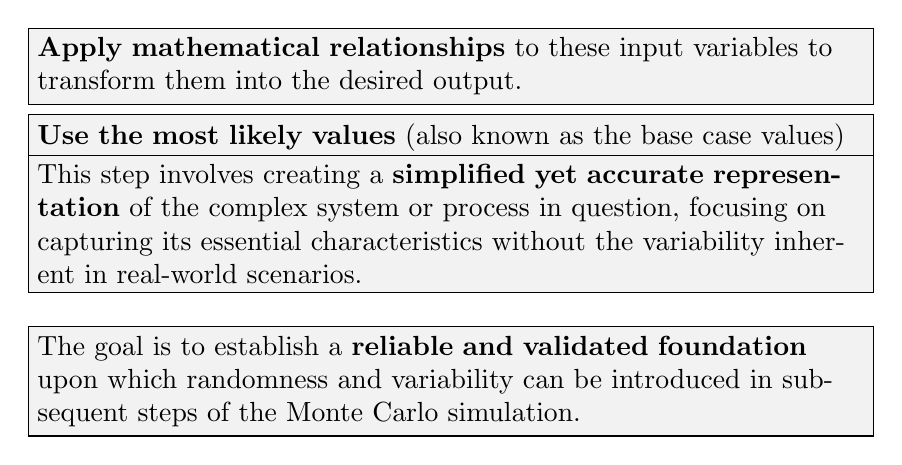
\begin{tikzpicture}
                \node<1-1>[draw, rectangle, black, fill=gray!10, text width=10.5cm](no1){\textbf{Start with a deterministic model} that closely resembles the real-world scenario being studied.};
                \node<2-2>[draw, rectangle, black, fill=gray!10, text width=10.5cm, below of=no1, yshift=-0.1cm](no2){\textbf{Use the most likely values} (also known as the base case values) for the input parameters of the model.};
                \node<3-5>[draw, rectangle, black, fill=gray!10, text width=10.5cm]{\textbf{Apply mathematical relationships} to these input variables to transform them into the desired output.};
                \node<4-5>[draw, rectangle, black, fill=gray!10, text width=10.5cm, yshift=-2cm]{This step involves creating a \textbf{simplified yet accurate representation} of the complex system or process in question, focusing on capturing its essential characteristics without the variability inherent in real-world scenarios.};
                \node<5-5>[draw, rectangle, black, fill=gray!10, text width=10.5cm, yshift=-4cm]{The goal is to establish a \textbf{reliable and validated foundation} upon which randomness and variability can be introduced in subsequent steps of the Monte Carlo simulation.};
            \end{tikzpicture}
        \end{center}
    \end{frame}

    \begin{frame}{Static Model Generation}
        \begin{center}
            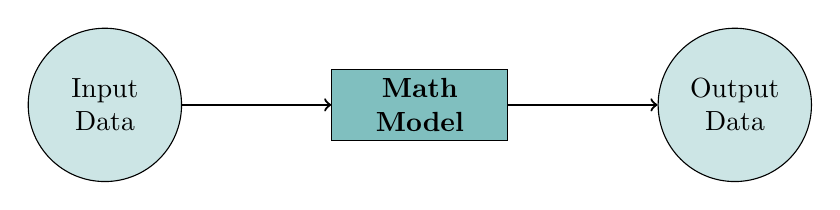
\begin{tikzpicture}
                \node[draw, rectangle, black, fill=teal!50, text width=2cm, text centered] (Begin) {\textbf{Math Model}};
                \node[draw, circle, fill=teal!20, text width=1.5cm, text centered, left of=Begin, xshift=-3cm, yshift=0cm] (Input) {Input Data};
                \node[draw, circle, fill=teal!20, text width=1.5cm, text centered, right of=Begin, xshift=3cm, yshift=0cm] (Output) {Output Data};
                \draw[black, thick, ->] (Input.east) -- (Begin.west);
                \draw[black, thick, ->] (Begin.east) -- (Output.west);
            \end{tikzpicture}
        \end{center}
    \end{frame}

    \subsection{Input Distribution Identification}
    \begin{frame}{Input Distribution Identification}
        \begin{columns}
            \begin{column}{.1\textwidth}
            \end{column}
            \begin{column}{0.9\textwidth}
                \begin{itemize}
                    \item Add the risk components
                    \item The stochastic nature of the input variables
                    \item Identify the underlying distributions if any,\\ which govern the input variables 
                    \item Needs historical data for the input variables
                \end{itemize}   
            \end{column}
        \end{columns}     
    \end{frame}

    \begin{frame}{Input Distribution Identification}
        \begin{figure}
            \centering
            \includegraphics[width=0.6\textwidth]{figures/log.jpeg}
            \caption{Log-Normal Distribution}
            \label{fig:log}
        \end{figure}
    \end{frame}

    \begin{frame}{Input Distribution Identification}
        \begin{figure}
            \centering
            \includegraphics[width=0.7\textwidth]{figures/normal.jpg}
            \caption{Standard Normal Distribution}
            \label{fig:normal}
        \end{figure}
    \end{frame}

    \begin{frame}{Statistical Procedures to Identify Input Distributions}
        \vspace{1em}
        Method of Maximum Likelihood (ML)
        \begin{itemize}
            \item<1->[-] Sample data drawn is independent and identically distributed (iid)
            \item<2->[-] Let the sample drawn from the distribution be $x_1, x_2,\ldots, x_n$. Then the likelihood of getting the sample from the distribution is given by $L(\theta)=f\theta (x_1, x_2,\ldots, x_n |\theta)$
            \item<3->[-] Given the independence of each of the data points, this can  be expanded to the equation $L(\theta)=\prod_{i=1}^{n}f\theta(x_i|\theta)$
            \item<4->[-] Finding the value of $\theta$ so that the value of $L(\theta)$ can be maximized 
        \end{itemize}
    \end{frame}

    \begin{frame}{Goodness-of-Fit  Statistics}
        The correctness of fitting a dataset to a distribution.
        \begin{itemize}
            \item Chi-square Test 
            \item Kolmogorov-Smirnov Statistic (KS)
            \item The Quadratic Statistics
        \end{itemize}
    \end{frame}

    % \subsection{Random Variable Generation}
    % \begin{frame}{Random Variable Generation}
    %     \vspace{1em}
    %     \textbf{Inverse Transformation Method}
    %     \begin{itemize}
    %         \item<1->[-] Let $X$ be a continuous random variate (which we want to generate) following a PDF function $f$. 
    %         \item<2->[-] Let the cumulative probability distribution function (CDF) for the variate be denoted by $F$, which is continuous and strictly increasing in $(0,1)$. 
    %         \item<3->[-] Let $F^{-1}$ denote the inverse of the function $F$. Then, the following two steps will generate a random number $X$ from the PDF $f$. 
    %         \begin{itemize}
    %             \item[i.] Generate $U \sim U(0,1)$
    %             \item[ii.] Return $X = F^{-1}(U)$
    %         \end{itemize}
    %     \end{itemize} 
    % \end{frame}

    % \begin{frame}{Random Variable Generation}
    %     \begin{figure}
    %         \centering
    %         \includegraphics[width=0.8\textwidth]{figures/image.png}
    %     \end{figure}
    % \end{frame}

    \subsection{Analysis and Decision Making}
    \begin{frame}{Analysis and Decision Making}
        \vspace{2em}
        \begin{itemize}
            \item<1-> \textbf{Calculating Trial Outputs:} the simulation model calculates trial values for the output variable(s). 
            \item<2-> \textbf{Averaging Outputs:} Determining expected values by averaging trial outputs.
            \item<3-> \textbf{Visualizing Distribution:} Creating frequency histograms to approximate the probability density function.
            \item<4-> \textbf{Empirical Distribution Analysis:} Using output values to calculate percentiles and other statistics directly.
            \item<5-> \textbf{Fitting Theoretical Distributions:} Optionally fitting output values to known distributions to develop confidence bands.
            \item<6-> \textbf{Improving Precision:} More number of trials enhances the accuracy of expected values and distribution approximations.
        \end{itemize}
    \end{frame}

    \begin{frame}{Basic statistical analysis for output values}
        \begin{center}
            \textbf{Mean} $\bar{x} = \frac{1}{n} \sum_{i=1}^{n} x_i$\\
            \vspace{1em}
            \textbf{Median} = $50^{th}$ Percentile\\
            \vspace{1em}
            \textbf{Standard Deviation} $\sigma = \sqrt{\frac{1}{N-1} \sum_{i=1}^{n} (x_i - \bar{x})^2}$\\
            \vspace{1em}
            \textbf{Variance} $\sigma^2 = \frac{1}{N-1} \sum_{i=1}^{n} (x_i - \bar{x})^2$\\
            \vspace{1em}
            \textbf{Skewness} = $\frac{\sum_{i=1}^{n} (x_i - \bar{x})^3}{(N-1)s^3}$\\
            \vspace{1em}
            \textbf{Kurtosis} = $\frac{\sum_{i=1}^{n} (x_i - \bar{x})^4}{(N-1)s^4}-3$
        \end{center}
    \end{frame}

    \section{Visualizing steps of Monte Carlo}
    \begin{frame}[fragile]{Visualizing All the steps of Monte Carlo}
        \begin{figure}
            \centering
            \includegraphics[width=\linewidth]{figures/code1.png}
        \end{figure}
    \end{frame}

    \begin{frame}{Visualizing steps of Monte Carlo}
        \begin{figure}
            \centering
            \includegraphics[width=0.8\linewidth]{figures/graph1.png}
        \end{figure}
    \end{frame}

    \begin{frame}{Visualizing steps of Monte Carlo}
        \begin{figure}
            \centering
            \includegraphics[width=\linewidth]{figures/code2.png}
        \end{figure}
    \end{frame}

    \begin{frame}{Visualizing steps of Monte Carlo}
        \begin{figure}
            \centering
            \includegraphics[width=0.8\linewidth]{figures/fig.png}
        \end{figure}
    \end{frame}

    \begin{frame}{Visualizing steps of Monte Carlo}
        \begin{figure}
            \centering
            \includegraphics[width=\textwidth]{figures/code3.png}
        \end{figure}
    \end{frame}

    \begin{frame}{Visualizing steps of Monte Carlo}
        \begin{figure}
            \centering
            \includegraphics[width=0.8\linewidth]{figures/fig2.png}
        \end{figure}
    \end{frame}

    \section{Application of Monte Carlo}
    \begin{frame}{A Simple Example - Calculate $\pi$}
        \begin{center}
            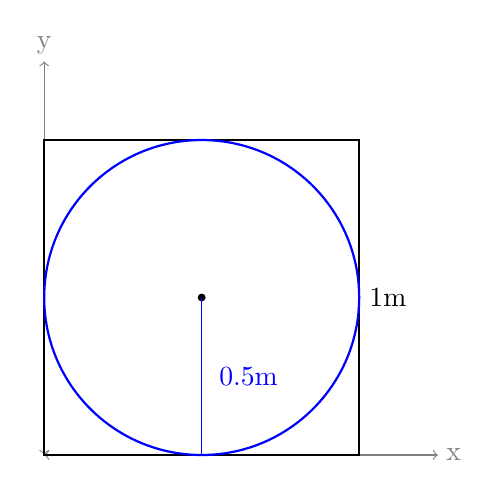
\begin{tikzpicture}
                \draw[gray, <->] (0, 0) -- (5, 0) node[xshift=2mm] {x};
                \draw[gray, <->] (0, 0) -- (0, 5) node[yshift=2mm] {y};
                \draw[black, thick] (0, 0) rectangle (4, 4) node[midway, right, xshift=20mm] {1m};
                \draw[blue, thick] (2, 2) circle (2);
                \fill[black] (2, 2) circle (0.05);
                \draw[blue] (2, 2) -- (2, 0) node[midway, right, xshift=1mm] {0.5m};
            \end{tikzpicture}
        \end{center}
        \begin{center}
            $\frac{A_{Circle}}{A_{Square}}=\frac{\pi (0.5)^2}{1^2}=\frac{\pi}{4}$
        \end{center}
    \end{frame}

    \begin{frame}{A Simple Example - Calculate $\pi$}
        \begin{center}
            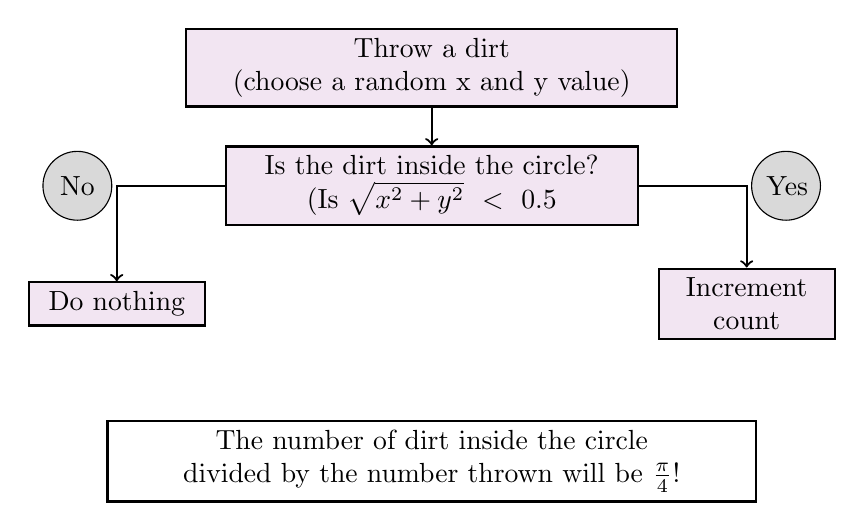
\begin{tikzpicture}
                \node<1->[draw, rectangle, black, fill=violet!10, thick, text width=6cm, text centered] (Begin) {Throw a dirt \\(choose a random x and y value)};
                \node<2->[draw, rectangle, black, fill=violet!10, thick, text width=5cm, text centered, below of=Begin, yshift=-0.5cm] (Decision) {Is the dirt inside the circle? \\(Is $\sqrt{x^2+y^2}<0.5$};
                \node<3->[draw, rectangle, black, fill=violet!10, thick, text width=2cm, text centered, left of=Decision, xshift=-3cm, yshift=-1.5cm] (No) {Do nothing};
                \node<4->[draw, rectangle, black, fill=violet!10, thick, text width=2cm, text centered, right of=Decision, xshift=3cm, yshift=-1.5cm] (Yes) {Increment count};
                \node<3->[draw, circle, black, fill=gray!30, text width=0.5cm, text centered, left of=Decision, xshift=-3.5cm, yshift=0cm] (no) {No};
                \node<4->[draw, circle, black, fill=gray!30, text width=0.5cm, text centered, right of=Decision, xshift=3.5cm, yshift=0cm] (yes) {Yes};
                \draw<2->[black, thick, ->](Begin.south) -- (Decision.north);
                \draw<4->[black, thick, ->](Decision.east) -| (Yes.north);
                \draw<3->[black, thick, ->](Decision.west) -| (No.north);
                \node<5->[draw, rectangle, black, thick, text width=8cm, text centered, below of=Decision, yshift=-2.5cm] (Decision) {The number of dirt inside the circle \\divided by the number thrown will be $\frac{\pi}{4}!$};
            \end{tikzpicture}
        \end{center}
    \end{frame}

    \begin{frame}{A Biological Example - Protein Folding}
        \begin{figure}
            \centering
            \includegraphics[width=\textwidth]{figures/protein.jpeg}
        \end{figure}
    \end{frame}
    
    \begin{frame}{A Biological Example - Protein Folding}
        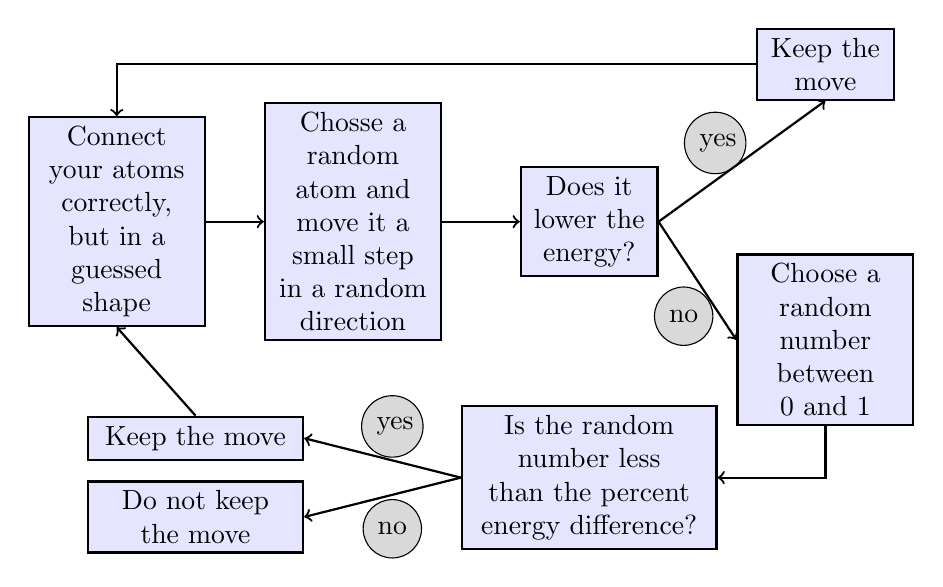
\begin{tikzpicture}
            \node<1->[draw, rectangle, black, fill=blue!10, thick, text width=2cm, text centered] (no1) {Connect your atoms correctly, but in a guessed shape};
            \node<2->[draw, rectangle, black, fill=blue!10, thick, text width=2cm, text centered, right of=no1, xshift=2cm, yshift=0cm] (no2) {Chosse a random atom and move it a small step in a random direction};
            \node<3->[draw, rectangle, black, fill=blue!10, thick, text width=1.5cm, text centered, right of=no2, xshift=2cm, yshift=0cm] (no3) {Does it lower the energy?};
            \node<4->[draw, circle, black, fill=gray!30, text width=0.4cm, text centered, right of=no3, xshift=0.6cm, yshift=1cm] (y) {yes};
            \node<6->[draw, circle, black, fill=gray!30, text width=0.4cm, text centered, right of=no3, xshift=0.2cm, yshift=-1.2cm] (y) {no};
            \node<4->[draw, rectangle, black, fill=blue!10, thick, text width=1.5cm, text centered, right of=no3, xshift=2cm, yshift=2cm] (no4) {Keep the move};
            \node<6->[draw, rectangle, black, fill=blue!10, thick, text width=2cm, text centered, right of=no3, xshift=2cm, yshift=-1.5cm] (no5) {Choose a random number between 0 and 1};
            \node<7->[draw, rectangle, black, fill=blue!10, thick, text width=3cm, text centered, left of=no5, xshift=-2cm, yshift=-1.75cm] (no6) {Is the random number less than the percent energy difference?};
            \node<8->[draw, rectangle, black, fill=blue!10, thick, text width=2.5cm, text centered, left of=no6, xshift=-4cm, yshift=0.5cm] (no7) {Keep the move};
            \node<10->[draw, rectangle, black, fill=blue!10, thick, text width=2.5cm, text centered, left of=no6, xshift=-4cm, yshift=-0.5cm] (no8) {Do not keep the move};
            \node<8->[draw, circle, black, fill=gray!30, text width=0.4cm, text centered, left of=no6, xshift=-1.5cm, yshift=0.65cm] (y) {yes};
            \node<10->[draw, circle, black, fill=gray!30, text width=0.4cm, text centered, left of=no6, xshift=-1.5cm, yshift=-0.65cm] (y) {no};
            \draw<2->[black, thick, ->](no1.east) -- (no2.west);
            \draw<3->[black, thick, ->](no2.east) -- (no3.west);
            \draw<4->[black, thick, ->](no3.east) -- (no4.south);
            \draw<6->[black, thick, ->](no3.east) -- (no5.west);
            \draw<5->[black, thick, ->](no4.west) -| (no1.north);
            \draw<7->[black, thick, ->](no5.south) |- (no6.east);
            \draw<9->[black, thick, ->](no7.north) -- (no1.south);
            \draw<8->[black, thick, ->](no6.west) -- (no7.east);
            \draw<10->[black, thick, ->](no6.west) -- (no8.east);
        \end{tikzpicture}
    \end{frame}

    \begin{frame}{Monte Carlo Simulation of Polypeptide Chain Folding, 2015}
        \begin{table}[h]
            \centering
            \begin{tabular}{cc}
                \includegraphics[width=0.45\textwidth]{figures/ap1.png} &  \includegraphics[width=0.45\textwidth]{figures/ap3.png} \\
                \includegraphics[width=0.45\textwidth]{figures/ap4.png} &  \includegraphics[width=0.45\textwidth]{figures/ap6.png} \\
            \end{tabular}
        \end{table}
    \end{frame}

    % \begin{frame}{Monte Carlo Simulation of Polypeptide Chain Folding, 2015}
    %     \begin{figure}
    %         \centering
    %         \includegraphics[width=\textwidth]{figures/ap1.png}
    %     \end{figure}
    % \end{frame}
    % \begin{frame}{Monte Carlo Simulation of Polypeptide Chain Folding, 2015}
    %     \begin{figure}
    %         \centering
    %         \includegraphics[width=\textwidth]{figures/ap2.png}
    %     \end{figure}
    % \end{frame}
    % \begin{frame}{Monte Carlo Simulation of Polypeptide Chain Folding, 2015}
    %     \begin{figure}
    %         \centering
    %         \includegraphics[width=\textwidth]{figures/ap3.png}
    %     \end{figure}
    % \end{frame}
    % \begin{frame}{Monte Carlo Simulation of Polypeptide Chain Folding, 2015}
    %     \begin{figure}
    %         \centering
    %         \includegraphics[width=\textwidth]{figures/ap4.png}
    %     \end{figure}
    % \end{frame}
    % \begin{frame}{Monte Carlo Simulation of Polypeptide Chain Folding, 2015}
    %     \begin{figure}
    %         \centering
    %         \includegraphics[width=\textwidth]{figures/ap5.png}
    %     \end{figure}
    % \end{frame}
    % \begin{frame}{Monte Carlo Simulation of Polypeptide Chain Folding, 2015}
    %     \begin{figure}
    %         \centering
    %         \includegraphics[width=\textwidth]{figures/ap6.png}
    %     \end{figure}
    % \end{frame}
    % \begin{frame}{Monte Carlo Simulation of Polypeptide Chain Folding, 2015}
    %     \begin{figure}
    %         \centering
    %         \includegraphics[width=\textwidth]{figures/ap7.png}
    %     \end{figure}
    % \end{frame}
    % \begin{frame}{Monte Carlo Simulation of Polypeptide Chain Folding, 2015}
    %     \begin{figure}
    %         \centering
    %         \includegraphics[width=\textwidth]{figures/ap8.png}
    %     \end{figure}
    % \end{frame}
    % \begin{frame}{Monte Carlo Simulation of Polypeptide Chain Folding, 2015}
    %     \begin{figure}
    %         \centering
    %         \includegraphics[width=\textwidth]{figures/ap9.png}
    %     \end{figure}
    % \end{frame}
    % \begin{frame}{Monte Carlo Simulation of Polypeptide Chain Folding, 2015}
    %     \begin{figure}
    %         \centering
    %         \includegraphics[width=\textwidth]{figures/ap10.png}
    %     \end{figure}
    % \end{frame}

    \section{Summary}
    \begin{frame}{Summary}
        \vspace{2em}
        \begin{itemize}
            \item <1-> Monte Carlo (MC) methods use random numbers to solve problems that cannot be solved any other way.
            \item <2-> Used in a variety of fields:
            \begin{itemize}
                \item[-] Physics
                \item[-] Biology
                \item[-] Geosciences
                \item[-] Finance
                \item[-] \dots
            \end{itemize}
            \item <3-> The versatility and efficiency of Monte Carlo algorithms make them an indispensable tool for tackling computationally challenging problems across diverse domains.
        \end{itemize}
    \end{frame}

    \section{Reference}
    \begin{frame}{References}
        \bibliographystyle{unsrt}
        \bibliography{ref}
    \end{frame}

    \begin{frame}{Conclusion}
        \begin{center}
            \Huge T\huge HANK \Huge Y\huge OU\Huge!\\
            \vspace{1em}
            \Large Any Questions?
        \end{center}
    \end{frame}

\end{document}